% Amplitude-estimation circuit around the peak-load oracle (TikZ); included from main.tex
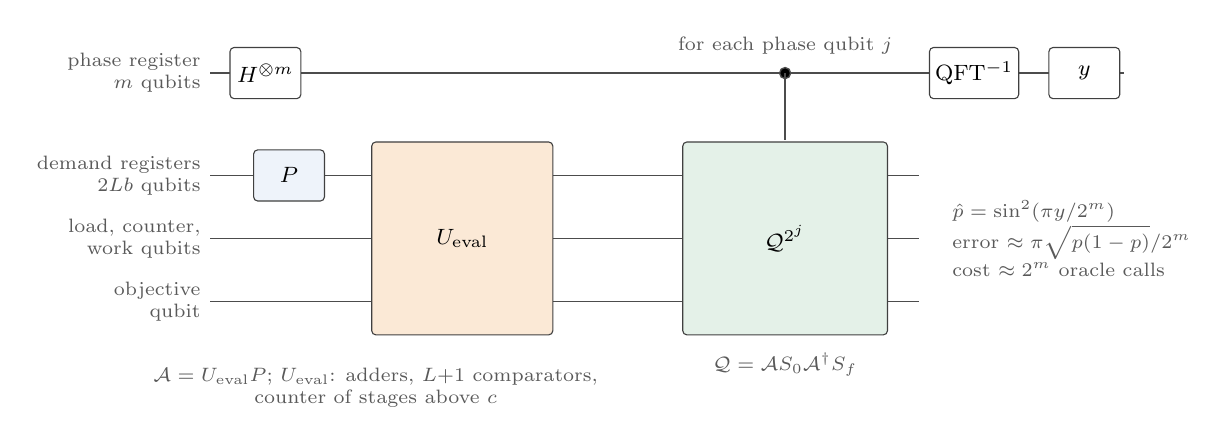
\begin{tikzpicture}[
  font=\footnotesize, x=1cm, y=1cm,
  g/.style={draw=black!75, fill=white, rounded corners=1.5pt, minimum height=6.5mm, minimum width=9mm, inner sep=2pt, align=center},
  wire/.style={black!70, line width=0.5pt},
  lab/.style={font=\scriptsize, text=black!65}
]
\definecolor{cA}{HTML}{EEF3FA}\definecolor{cU}{HTML}{FBE9D6}\definecolor{cQ}{HTML}{E4F1E8}
\foreach \y/\t in {0/{phase register\\ $m$ qubits}, -1.3/{demand registers\\ $2Lb$ qubits}, -2.1/{load, counter,\\ work qubits}, -2.9/{objective\\ qubit}} {
  \draw[wire] (0.3,\y) -- (\ifdim\y pt=0pt 11.9\else 9.3\fi,\y);
  \node[left, lab, align=right] at (0.3,\y) {\t};
}
\node[g] at (1.0,0) {$H^{\otimes m}$};
\node[g, fill=cA] at (1.3,-1.3) {$P$};
\node[g, fill=cU, minimum height=2.45cm, minimum width=2.3cm] at (3.5,-2.1) {$U_{\rm eval}$};
\node[lab, align=center] at (2.4,-4.0) {$\mathcal A=U_{\rm eval}P$; $U_{\rm eval}$: adders, $L{+}1$ comparators,\\ counter of stages above $c$};
\draw[wire, fill=black] (7.6,0) circle (0.07);
\draw[wire] (7.6,0) -- (7.6,-0.85);
\node[g, fill=cQ, minimum height=2.45cm, minimum width=2.6cm] at (7.6,-2.1) {$\mathcal Q^{2^{j}}$};
\node[lab] at (7.6,0.35) {for each phase qubit $j$};
\node[g] at (10.0,0) {QFT$^{-1}$};
\node[g] at (11.4,0) {$y$};
\node[lab, align=center] at (7.6,-3.7) {$\mathcal Q=\mathcal A S_0\mathcal A^{\dagger}S_f$};
\node[lab, align=left, anchor=west] at (9.6,-2.1) {$\hat p=\sin^2(\pi y/2^{m})$\\ error $\approx\pi\sqrt{p(1-p)}/2^{m}$\\ cost $\approx 2^{m}$ oracle calls};
\end{tikzpicture}
